\documentclass[conference]{IEEEtran}
\newtheorem{definition}{Definition}
\usepackage{dblfloatfix}
%\IEEEoverridecommandlockouts
% The preceding line is only needed to identify funding in the first footnote. If that is unneeded, please comment it out.
\usepackage{cite}
\usepackage{amsmath,amssymb,amsfonts}
\usepackage{algorithmic}
\usepackage{graphicx}
\usepackage{textcomp}
\usepackage{xcolor}
%\def\BibTeX{{\rm B\kern-.05em{\sc i\kern-.025em b}\kern-.08em
%		T\kern-.1667em\lower.7ex\hbox{E}\kern-.125emX}}

\usepackage{algorithm}
\usepackage{changepage}
\usepackage{comment}
%\usepackage[title]{appendix}
\usepackage{hyperref}
%\usepackage{caption}
%\usepackage[font=scriptsize]{subcaption}
\usepackage{color} % added by Bayzid
\newcommand{\commentA}[1]{{\color{red} #1}}
\newcommand{\commentM}[1]{{\color{blue} #1}}
\usepackage{subcaption}
\renewcommand{\algorithmiccomment}[1]{~{\scriptsize\ttfamily{/*#1*/}}}
\usepackage{enumitem}
\usepackage{multirow}
\usepackage{numprint}
%to squeeze space between sections, subsections and subsubsections
%\makeatletter
%\renewcommand\section{\@startsection{section}{1}{\z@}%
%	{-8\p@ \@plus -4\p@ \@minus -4\p@}%
%	{6\p@ \@plus 4\p@ \@minus 4\p@}%
%	{\normalfont\large\bfseries\boldmath
%		\rightskip=\z@ \@plus 8em\pretolerance=10000 }}
%\renewcommand\subsection{\@startsection{subsection}{2}{\z@}%
%	{-8\p@ \@plus -4\p@ \@minus -4\p@}%
%	{6\p@ \@plus 4\p@ \@minus 4\p@}%
%	{\normalfont\normalsize\bfseries\boldmath
%		\rightskip=\z@ \@plus 8em\pretolerance=10000 }}
%\renewcommand\subsubsection{\@startsection{subsubsection}{3}{\z@}%
%	{-4\p@ \@plus -4\p@ \@minus -4\p@}%
%	{-1.5em \@plus -0.22em \@minus -0.1em}%
%	{\normalfont\normalsize\bfseries\boldmath}}
%\makeatother
%\captionsetup{belowskip=-10pt}

\begin{document}
%
\title{Evolutionary Multi-objective Optimization Improves Phylogenomic Analyses}
%\title{Improving Accuracy of Species Tree Estimation by Employing Evolutionary Multi-objective Optimization}
%\author{\IEEEauthorblockN{Muhammad Ali Nayeem}
%	\IEEEauthorblockA{\textit{Department of CSE, BUET} \\
%		Dhaka, Bangladesh \\
%		ali\_nayeem@cse.buet.ac.bd}
%	\and
%	\IEEEauthorblockN{Md. Shamsuzzoha Bayzid}
%	\IEEEauthorblockA{\textit{Department of CSE, BUET} \\
%		Dhaka, Bangladesh \\
%		shams\_bayzid@cse.buet.ac.bd}
%	\and
%	\IEEEauthorblockN{Sakshar Chakravarty}
%	\IEEEauthorblockA{\textit{Department of CSE, BUET} \\
%		Dhaka, Bangladesh \\
%		saksharchakravarty5068@gmail.com}
%	\and
%	\IEEEauthorblockN{Mohammad Saifur Rahman}
%	\IEEEauthorblockA{\textit{Department of CSE, BUET} \\
%		Dhaka, Bangladesh \\
%		mrahman@cse.buet.ac.bd}
%	\and
%	\IEEEauthorblockN{M. Sohel Rahman}
%	\IEEEauthorblockA{\textit{Department of CSE, BUET} \\
%		Dhaka, Bangladesh \\
%		msrahman@cse.buet.ac.bd}
%}
\author{\IEEEauthorblockN{Muhammad Ali Nayeem\IEEEauthorrefmark{2}, Md. Shamsuzzoha Bayzid\IEEEauthorrefmark{2}, Sakshar Chakravarty\IEEEauthorrefmark{2}, Mohammad Saifur Rahman\IEEEauthorrefmark{2}\\ and M. Sohel Rahman\IEEEauthorrefmark{2}\IEEEauthorrefmark{1}}
	\IEEEauthorblockA{\IEEEauthorrefmark{2}Department of CSE, BUET, 
		Dhaka, Bangladesh}
	\IEEEauthorblockA{\IEEEauthorrefmark{1}Corresponding author, Email: msrahman@cse.buet.ac.bd}
%	\IEEEauthorblockA{\IEEEauthorrefmark{3}Starfleet Aca
%		demy, San Francisco, California 96678-2391\\
%		Telephone: (800) 555--1212, Fax: (888) 555--1212}
%	\IEEEauthorblockA{\IEEEauthorrefmark{4}Tyrell Inc.,
%		123 Replicant Street, Los Angeles, California 90210
%		--4321}
}

\maketitle              % typeset the header of the contribution
%
\begin{abstract}
	Species tree estimation from multi-locus data is complicated as biological processes can result in different loci having different evolutionary histories. Incomplete lineage sorting (ILS), modeled by the multi-species coalescent (MSC), is considered to be a dominant cause for gene tree incongruence. Various optimization criteria (e.g., quartet consistency, pseudo-likelihood, etc.) are statistically consistent under the MSC model, meaning that they return the true species tree with high probability given sufficiently large numbers of accurate gene trees. However, the number of genes is limited and estimating highly accurate gene trees is difficult. Therefore, even the statistically consistent methods may fail to reconstruct highly accurate trees under practical model conditions with limited numbers of genes and in the presence of gene tree estimation error. In this paper, we present an evolutionary multi-objective optimization (EMO) algorithm (SNOGA), a modified version of the popular NSGAII, which combines various optimization criteria to find a suitable search space containing highly accurate species trees. Our experimental results on a collection of simulated datasets demonstrate that SNOGA can lead us to a tree-space containing significantly better trees than the trees estimated by ASTRAL and MP-EST which are two of the most widely used methods. %\commentA{and their neighboring trees.}
	
	%The abstract should briefly summarize the contents of the paper in 15--250 words.
	
%	\keywords{Bioinformatics \and Phylogenomics  \and Multi-objective
%		optimization \and Evolutionary Algorithm.}
\end{abstract}

\begin{IEEEkeywords}
	Bioinformatics, Phylogenomics, Multi-objective
	optimization, Evolutionary Algorithm, insert
\end{IEEEkeywords} 
\section{Introduction}
\label{sec:intro}
% for bioinformatics community, we don't need this introduction about phylogeny; but for evocomp, we need this
In biological studies, evolutionary relationships between a group of organisms (usually called as taxa) are referred to as phylogeny. A hypothesis regarding such history is inferred in the form of a tree popularly known as the phylogenetic tree. A forking point in a phylogenetic tree depicts a historical speciation event that split a single population into two distinct species.  Knowledge discovered through analyzing such trees has benefited several branches of science including but not limited to medicine, forensics, bio-geography, epidemiology~\cite{felix2015phylogenetics}. 
A species tree represents the evolutionary relationships of a group of organisms. On the other hand, the phylogeny specific to a particular region of the genome (known as locus or gene) is termed as a gene tree~\cite{maddison1997gene}. A standard approach for species tree estimation uses multiple loci, then concatenates alignments for each locus
into a super-matrix based on the assumption that all genes have the same gene tree topology~\cite{huelsenbeck1996combining, de2007supermatrix}, which is then used to estimate a species phylogeny. When all the genes evolve down the same tree topology,  sequence-based statistical approaches such as maximum likelihood applied to the super-matrix are statistically consistent. 
However, gene trees may differ from each other, because genes duplicate, are lost or laterally transferred, or because alleles can coexist in populations spanning several speciation events~\cite{maddison1997gene}.
Therefore, concatenation (also known as combined analysis) can be statistically inconsistent~\cite{roch2015likelihood}, and can return incorrect trees with high confidence~\cite{kubatko-degnan-2007,edwards2007,leache-rannala,degiorgio2009}. Therefore, developing species tree estimation methods that take gene tree discordance into account has intrinsic value in phylogenomics.




Among the newer methods, perhaps the most popular ones belong to a family called ``summary methods''~\cite{bayzid2013naive}. They take the gene trees estimated from the individual genes as input and then find a species tree that best summarizes the gene trees under various optimization criteria. 
Because incomplete lineage sorting is
expected to occur under many biologically realistic conditions (e.g., rapid radiations)~\cite{jarvis2014whole}, statistically consistent coalescent-based species tree methods have been developed and are increasingly popular. 
Examples of such methods include
MP-EST~\cite{mpest}, *BEAST~\cite{heled-drummond}, NJst~\cite{njst}, BUCKy~\cite{larget-bioinf2010}, GLASS~\cite{glass}, STEM~\cite{stem}, SNAPP~\cite{snapp}, SVDquartets~\cite{svdquartet}, STEAC~\cite{steac},
ASTRAL~\cite{mirarab2014astral}, ASTRID~\cite{vachaspati2015astrid}, and STELAR~\cite{islam2019stelar}. Each of them optimizes a particular criterion that has been shown to be statistically consistent. For instance, ASTRAL tries to find a species tree by maximizing the number of quartets in the gene trees that are consistent with it. The quartet-score of the ASTRAL-estimated tree is expected to converge to the quartet-score of the true tree given sufficiently large numbers of true gene trees. However, with a limited number of genes and in the presence of gene tree estimation error, existing methods may \textit{overshoot} the criterion they try to optimize, and thus may deviate from the true tree. We have observed that (please see Section~\ref{subsec:observation}), in most of the cases, quartet-scores of the ASTRAL trees are more than the quartet-scores of the true trees. Similarly, MP-EST, which maximizes a pseudo-likelihood measure, tends to overestimate the amount of ILS present in the gene trees~\cite{statistical-binning,bayzid2015weighted}. Moreover, the performance of various optimization criteria varies with varying model conditions~\cite{mirarab2014evaluating,chou2015comparative}.


Therefore, optimizing a particular optimization criterion, despite being statistically consistent, may not always produce highly accurate trees. This phenomenon motivates us to apply evolutionary multi-objective optimization (EMO). An EMO algorithm evolves a population (i.e., a set of candidate solutions) by simultaneously optimizing multiple criteria end eventually outputs a collection of candidate solutions. In this paper, we focus on finding a tree-space by an EMO algorithm containing highly accurate trees under practical model conditions with limited numbers of estimated gene trees. 

Previously several researchers~\cite{villalobos2018memetic, santander2016performance, zambrano2016mo} successfully applied EMO approaches to infer phylogenetic trees from biological sequences. This is the first known study that aims to improve the accuracy of the species trees, estimated from a given set of gene trees, by multi-objective formulation. We show that if an appropriate EMO algorithm is employed to optimize different optimization criteria simultaneously, the final population is more likely to contain better species trees than the individual outputs of the existing methods.
%, santander2012inferring, cancino2007multi
%We developed an NSGAII~\cite{deb2002fast}, a popular EMO algorithm, based framework for species tree estimation. 
More importantly, we design a specially customized algorithm, namely, SNOGA (Summation of Normalized Objectives based Genetic Algorithm), by modifying a popular EMO algorithm, NSGAII~\cite{deb2002fast}. The final population of SNOGA contains better species trees than that of NSGAII.  %(Section~\ref{sec:method}).
We consider three optimization criteria: quartet consistency (ASTRAL), maximum pseudo-likelihood (MP-EST), and triplet consistency (STELAR). We assess the validity of our approach on a collection of challenging simulated datasets. Our results suggest that SNOGA can produce a tree-space which contains substantially more accurate trees than the trees estimated by optimizing the individual criterion. 

%Furthermore, we explored the SPR (subtree pruning and regrafting) neighborhood of ASTRAL and MP-EST estimated trees and showed that they do not contain the highly accurate trees that can be found in the population generated by SNOGA using multi-objective optimization.





\begin{comment}
%Then the super-matrix is analyzed using some sequence-based statistical approaches such as maximum likelihood. However, modern studies~\cite{zwickl2014disentangling, jarvis2014whole} show that the gene trees can be discordant with each other as well as with the species tree for various biological reasons. This observation has challenges the correctness of the traditional approach and thereby motivated the researchers to develop efficient methods to estimate species trees without concatenation. 

%To the best of our knowledge, this paper takes the first initiative to improve the accuracy of estimated species tree by existing summary methods by employing EMO algorithms.  In particular, here we make the following key
%contributions:
\begin{itemize}
\item We pick three optimization scores from three different methods (ASTRAL, STELAR and MP-EST) to be simultaneously optimized by an EMO algorithm (Section~\ref{sec:problem}).  
\item We developed an NSGA-II~\cite{deb2002fast}, a popular EMO algorithm, based framework. Also, based on obtained observations, we designed a custom genetic algorithm whose final population contains a better species tree than that of the NSGA-II (Section~\ref{sec:method}). 
\item Finally based on three simulated datasets, we examine the operation of the two EMO algorithms and then compare their performance with three existing methods (Section~\ref{sec:experiment}). 
\end{itemize}
\end{comment}


 
\section{Problem Description}
\label{sec:problem}
We are given a set of $M$ rooted binary trees as a collection gene trees each having $N$-taxon. We need to construct the species tree, a rooted binary tree with $N$-taxon, from these gene trees by simultaneously optimizing the following three objective functions:  
\begin{enumerate}[label=$F_\arabic*$)]        
	\item Maximize QT 
	\subitem {\scriptsize QT: number of consistent quartets (i.e., unrooted 4-taxon tree) between the species tree and the gene trees (used by ASTRAL\cite{mirarab2014astral})}
	\item Maximize TP
	\subitem {\scriptsize TP: number of consistent triplets (i.e., rooted 3-taxon tree) between the species tree and the gene trees (used by STELAR~\cite{islam2019stelar})}
	\item Maximize PL 
	\subitem {\scriptsize PL: pseudo-likelihood estimation of the species tree utilizing the underlying triplet distribution of the gene trees (used by MP-EST~\cite{mpest})}
\end{enumerate}
 To remain in line with the EMO literature and software frameworks, in what follows we have treated each objective as a minimization criterion. Unlike traditional multi-objective optimization problems (MOPs), here our goal is not only to effectively sampling the Pareto front (PF) because of the following two issues:
\begin{enumerate}[label=$I_\arabic*$]
	\item \label{item:i1} Optimizing an objective beyond a certain limit can lead the resultant species tree deviate from the true tree (please see Section~\ref{subsec:observation})
	%\item 
	\item \label{item:i2} A solution that is badly dominated at an early generation can still potentially evolve into a highly accurate tree at a later generation (also reported in~\cite{qu2010multi})
\end{enumerate}

%On the other hand, PF allows degrading an objective to achieve improvement in other objectives.
%The traditional definition of convergence is may not apply to this problem. 
%Therefore in this paper, we try to design a special-purpose EMO algorithm from NSGAII by replacing which can find a tree-space containing highly accurate species trees. 
%Each of the above functions (optimized by an existing method) has some ability to predict the species tree accuracy but none of them can necessarily lead towards the most accurate species tree. Therefore, optimizing them together, by an EMO algorithm, will generate a set of candidate solutions which is expected to contain a species tree that is more accurate than the output of the existing methods.
\section{Methodology}
\label{sec:method}
In this paper, we adapt NSGAII for species tree estimation by integrating problem-specific encoding, initialization, crossover and mutation. Moreover, we design a special purpose EMO algorithm by modifying NSGAII considering the issues mentioned in Section~\ref{sec:problem}. In this section, we discuss the design of our modified EMO algorithm (pseudo-code shown in Algorithm~\ref{alg:nossga}) along with its different components. In what follows, the following definition will be useful. %associated with the problem 

\begin{definition}\label{def:domination_threshold}
	\small
	We call the worst value of a particular objective in the obtained PF of a certain generation as the \textbf{domination threshold} for that objective at that generation.
\end{definition}

\subsection{Algorithm Design}
One idea to resolve issue~\ref{item:i1}, could be to enforce the EMO algorithm being applied to maintain a population that contains some solutions having objective values slightly below the domination threshold (Definition~\ref{def:domination_threshold}). However, any such algorithm, in general, would continue optimizing one objective to a great extent even at the loss of some other objectives (resulting in issue~\ref{item:i1}) which may be detected through a change in sign of correlation coefficient (positive to negative)  between a pair of objectives as the generation changes. 
Therefore, we modify NSGAII to tackle issue~\ref{item:i1} in a better way than the original NSGAII in addition to resolving issue~\ref{item:i2}.  

\begin{equation}\label{eqn:nos}
\small
SNO(x) = \sum_{i=1}^{3} \frac{F_i(x)-z_i^{min}}{z_i^{max}-z_i^{min}}
\end{equation}
Here $x$ is a candidate solution (i.e., species tree) and $z_i^{min}$ ($z_i^{max}$) is the minimum (maximum) value of $i^{th}$ objective $F_i$ observed so far during the search process.

To overcome issue~\ref{item:i2}, we avoid the concept of non-domination while selecting solutions to form the population for the next generation (line~\ref{line:next_pop1}-\ref{line:next_pop2} of Algorithm~\ref{alg:nossga}). Instead, we sort solutions (line~\ref{line:sort_nos} of Algorithm~\ref{alg:nossga}) based on the summation of normalized objective (SNO) values as defined by the $SNO()$ function in Equation~\ref{eqn:nos}. That is why, we refer to our algorithm as SNOGA, i.e, Summation of Normalized Objectives based Genetic Algorithm. We are inspired by~\cite{qu2010multi} where a similar strategy was utilized to design an EMO algorithm. Moreover, as an attempt to address issue~\ref{item:i1}, we will not allow the selection of individuals that may arise conflict (negative correlation coefficient) between any pair of objectives. We accomplish this by using the tournament selection~\cite{goldberg1991comparative} based on $SNO()$ (line~\ref{line:tournament_nos}) while forming the offspring population.
%instead of the default binary tournament. 
Because we expect that selection pressure based on $SNO()$ will prefer those solutions that achieve reasonably well values across all objective than those solutions which are optimized along one objective heavily at the cost of other objectives. This feature might help us to resolve or at least lessen issue~\ref{item:i1} compared to the original NSGAII algorithm (this is supported by results presented in Section~\ref{sec:experiment}). %at least better than NSGAII. %as well as address issue~\ref{item:i2} that NSGAII cannot handle. 

Additionally, we always randomly choose one from among multiple solutions having the same $SNO()$ value (line \ref{line:diversity}) to help maintain the diversity of solutions. Also, we attempt to preserve diversity by using the crowding distance concept of NSGAII, albeit in a different way than NSGAII, by keeping some sparsely spaced (in the objective space) solutions having poor $SNO()$ values (line~\ref{line:crowding_s}-\ref{line:crowding_e}) in the population. In addition to doing tournament selection (as mentioned above), unlike NSGAII, we also use the random selection (line~\ref{line:random_selection}) to ensuring the participation of a few poor solutions (in terms of $SNO()$) in the offspring generating process. This increases the exploration capability of SNOGA to help escape local optima. Moreover, we expect this feature to aid in addressing issue~\ref{item:i2} as well.


%It optimizes three objectives, with certain attention to the nature of the problem, and generates a tree-space that contains high-quality species trees. 
%We also apply NSGAII, using the same crossover, mutation and initialization method as the SNOGA, to approximate the PF by optimizing the three objectives. 

\begin{algorithm}[!htbp]
	\scriptsize
	\caption{SNOGA}
	\textbf{Input:} $m_g$ (max. generations), $p_s$ (population size), $c_r$ (crossover rate), $m_r$ (mutation rate), $t_s$ (tournament size)\\
	\textbf{Output:} $P$ (A list of $p_s$ candidate solutions i.e., species trees)
	\begin{algorithmic}[1]\label{alg:nossga}
		\STATE{$P \gets$ population\_initialization($N$)} \COMMENT{Sec.~\ref{subsec:init}}
		\STATE{For each solution in $ P $, evaluate the objective functions and $SNO()$ function} \COMMENT{using Eqn.\ref{eqn:nos}}
		%\STATE{For each solution $x$ in $ P $, calculate SNO($x$)}
		\STATE{$g \gets 0$} \COMMENT{generation counter}
		\WHILE{ $g < m_g$}
		\STATE{$Q \gets \emptyset$} \COMMENT{offspring population, an empty list that can hold $p_s$ solutions}
		\FOR{$i \leftarrow 1$ to $p_s$}    %\label{mainLoop}    
		\STATE{$S_1 \gets$ tournament\_selection($P$, $t_s$)} \COMMENT{based on value of $SNO()$ function} \label{line:tournament_nos}
		\STATE{$S_2 \gets$ random\_selection($P$)} \label{line:random_selection}
		\STATE{$x \gets$ mutation(crossover($S_1, S_2, c_r$), $m_r$)}\COMMENT{Sec.~\ref{subsec:crossver}, \ref{subsec:mutation}}
		\STATE{$\!\!$Add $x$ to tail($Q$)}
		%\STATE{Generate an offspring by applying crossover on $S_1, S_2$, then mutate the offspring and append the resultant solution to $Q$}        
		\ENDFOR    
		\STATE{For each solution in $ Q $, evaluate the objective functions and $SNO()$ function }
		\STATE{$ R \gets P \cup Q$} \COMMENT{$R$ is a list holding $2p_s$ solutions}
		%\STATE{For each solution $x$ in $ R $, calculate SNO($x$)}
		\STATE{Sort the members of $ R $ in ascending order of $SNO()$ values} \COMMENT{ascending because all objectives are treated as minimization}\label{line:sort_nos} \label{line:nos}
		\STATE{$P \gets \emptyset$, Remove the solution from head($R$) and add it to tail($P$)} \label{line:next_pop1}
		%\STATE{$P[1] \gets R[1]$}
		%\STATE{$i \gets 2$}
		\FOR{$i \leftarrow 2$ to $p_s$}    %\label{mainLoop}  
		\STATE{Remove the solution from head($R$) and store it in $x$}    %\COMMENT{each element is shifted left by 1 position }   
		\STATE{\textbf{if} $SNO$($x$) $\ne$ $SNO$(solution at tail($P$)), \textbf{then} Add $x$ to tail($P$) }    \label{line:diversity}
		
		\ENDFOR    \label{line:next_pop2}
		%            \FOR{$i \gets 1$ to $N$}    %\label{mainLoop}    
		%                \IF{ SNO($R[i]) \ge P[i-1]$)}
		%                    \STATE{$P[i] \gets R[i]$}
		%                \ENDIF
		%                \STATE{Remove $R[i]$ from $R$}        
		%            \ENDFOR    
		%\STATE{For each remaining solution in $ R $, calculate the crowding distance}\label{line:crowding_s}
		\STATE{Sort the members of $ R $  in descending order of their crowding distance~\cite{deb2002fast} in $R$} \label{line:crowding_s}
		\STATE{Fill-up the remaining solutions for $P$ from the top of $R$}\label{line:crowding_e}
		\STATE{$g \gets g + 1$}
		\ENDWHILE
		\STATE{\textbf{return} $P$}
	\end{algorithmic}
\end{algorithm}

\subsection{Crossover}\label{subsec:crossver}
We use Prune-Delete-Graft (PDG)~\cite{villalobos2018memetic} as the crossover operator which generates one tree (i.e., offspring) from two parents. At first, it takes a random sub-tree from one of the parents. Then, it inserts the selected sub-tree in the other parent at a
randomly selected insertion point. Finally, it deletes duplicated species from the second tree and returns it as the output.

\subsection{Mutation} \label{subsec:mutation}
Our mutation operator applies one of the three widely used tree rearrangement strategies~\cite{felsenstein2004inferring}: (i) Nearest Neighbour
Interchange (NNI), (ii) Sub-tree Pruning and Re-grafting (SPR) and (iii) Tree Bisection and Reconnection (TBR). Each of them is selected randomly with equal probability. NNI exchanges sub-trees from an arbitrary internal branch to obtain a new tree. On the other hand, SPR picks a random sub-tree from a tree, removes it and then re-grafts it in a random position to generate a new tree. And TBR is a combination of SPR and NNI.

\subsection{Population Initialization}\label{subsec:init}
We generate the required number of solutions for the initial population by utilizing the given set of gene trees. To produce a single solution, we randomly pair two gene trees and apply our crossover operator on them with probability 1.0. 


\subsection{Implementation Notes}
We encode species tree using \textit{TreeTemplate} class provided by BIO++~\cite{gueguen2013bpp} which is a collection of C++ libraries for Bioinformatics. To implement NSGAII and SNOGA, we use a C++ framework for EMO, jMetalCpp~\cite{lopez2013jmetalcpp}. We reuse the implementation of PDG, NNI, SPR and TBR from~\cite{zambrano2016mo} after fixing some minor bugs therein. Furthermore, we evaluate each objective (QT/TP/PL) using a feature provided by each method (ASTRAL/STELAR/MP-EST) to score an existing species tree. Thus for each candidate solution, we invoke the executable of a particular method to evaluate an objective.
%\footnote{\url{https://github.com/jMetal/jMetalCpp}}
\begin{comment}
\subsection{Objective Evaluation}
Each method (ASTRAL, STELAR or MP-EST) provides an option to score an existing species tree. We used this feature to enable to evaluate the objectives. Thus for each candidate species tree, we invoke the executable of a particular method (ASTRAL/STELAR/MP-EST) to evaluate an objective. %We converted each objective into minimization to conform 
%We evaluated each objective by executing the method that 
%: invoke java executable
%MP-EST: Maximize branch length, c++ executable
\end{comment}
\begin{figure*}[!htbp]
	\begin{adjustwidth}{-4cm}{-3cm}
		\centering    
		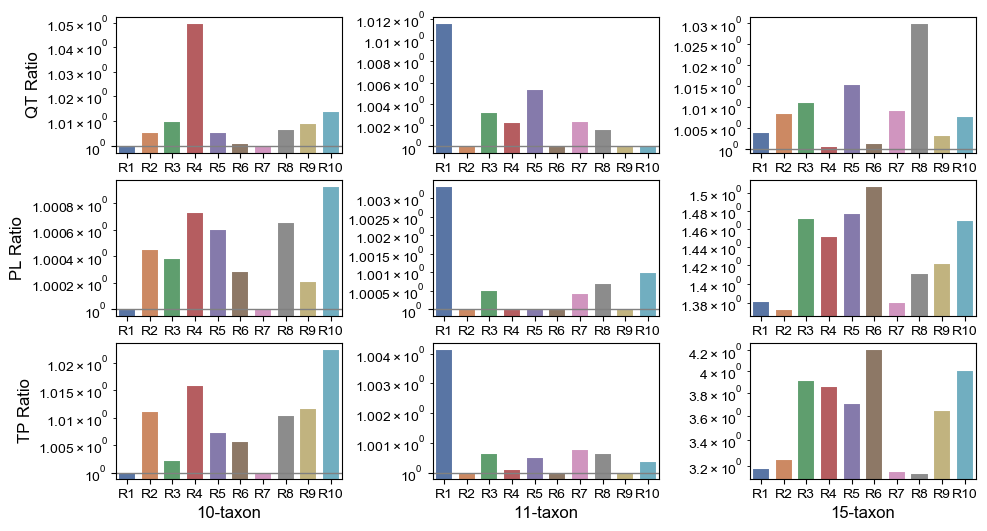
\includegraphics[width=1\textwidth]{Figure/tool_ratio}
	\end{adjustwidth}
	\caption{The issue of overshooting the optimization criterion beyond the true tree by existing methods. Each row shows the ratio of scores (QT/PL/TP), optimized by a particular method (ASTRAL/MP-EST/STELAR), of the true tree to that of the estimated tree by the same method.} \label{fig:tool_ratio}
\end{figure*}

\section{Experimental Studies}
\label{sec:experiment}
We examine the difference in the operation of NSGAII and SNOGA and evaluate their performance in comparison with three existing methods (ASTRAL, MP-EST and STELAR). ASTRAL and MP-EST are two of the most widely used and accurate summary methods~\cite{islam2019stelar}. We used three simulated datasets: 10-taxon (\#estimated gene tree: 200)~\cite{bayzid2015weighted}, 11-taxon (\#estimated gene tree: 50)~\cite{chung2011comparing} and 15-taxon (\#estimated gene tree: 100)~\cite{statistical-binning}. Each of them has 10 replicates (R1 to R10). We used False Negative (FN) rate~\cite{bayzid2013naive} to measure the accuracy of the estimated species tree. FN rate expresses the fraction of edges present in the true species tree (Provided with the dataset) but missing in the estimated tree. Thus the calculated FN rate of the solutions finally returned by an algorithm reflects the actual performance of that algorithm concerning the application (i.e., species tree estimation).%previously studied

For NSGAII and SNOGA, we carried out 15 independent runs due to their stochastic nature. We collected the trees estimated by ASTRAL, STELAR and MP-EST from~\cite{islam2019stelar}. They ran the exact version of ASTRAL and STELAR, which are guaranteed to return the globally optimal tree. And for MP-EST, they ran with 10 random starting points and selected the species tree with the best PL value.   



\subsection{Overshooting of Optimization Criterion}
\label{subsec:observation}
At first, we present an important observation that essentially motivated us to tackle the problem of species tree estimation as a MOP. As we mentioned in Section~\ref{sec:intro}, existing methods may overshoot the criterion they try to optimize, and thus may deviate from the true tree. In Fig.~\ref{fig:tool_ratio}, we summarize our observations for three methods (ASTRAL, MP-EST and STELAR) on 10 replicates of our selected datasets. Here, the top row shows the ratio of quartet-scores (QT) of the true trees to quartet-scores (QT) of the ASTRAL-estimated trees. Likewise, the middle row shows the pseudo-likelihood (PL) ratio of the true trees and MP-EST estimated trees and the bottom row does the same with the triplet (TP) ratio of STELAR. As we treat each objective as a minimization task, ideally these ratios should be 1 (marked as a gray horizontal line in each plot). However, we find that in most of the cases the ratio is greater than 1 implying that the results have been over-optimized. %And for 15-taxon (third column of Fig.~\ref{fig:tool_ratio}), we 


\subsection{NSGAII vs. SNOGA}
Now we closely inspect the behavioral difference between NSGAII and SNOGA to find out how SNOGA addresses the two issues (mentioned in Section~\ref{sec:problem}) in comparison with NSGAII. To ensure a level playing field, we executed both algorithms with the same configuration (independent run: 15, population size: 100, maximum generations: 99, crossover rate: 0.3, mutation rate: 1.0). For SNOGA, we use tournament size 10.

\begin{figure*}[!htbp]
	%\scriptsize
	\centering
	%\begin{adjustwidth}{-1cm}{-1cm}
		\begin{subfigure}[b]{0.3\textwidth}
			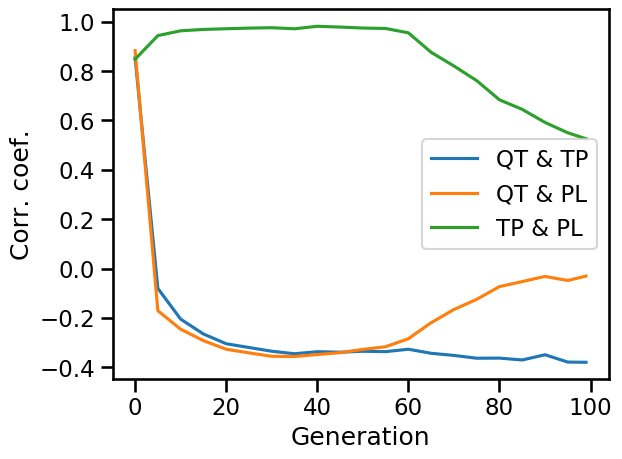
\includegraphics[width=\textwidth]{Figure/10-taxon_NSGAII_corr_plot}
			\caption{NSGAII: 10-taxon}
			%\label{fig:con_pr06}
		\end{subfigure}%
		\begin{subfigure}[b]{0.3\textwidth}
			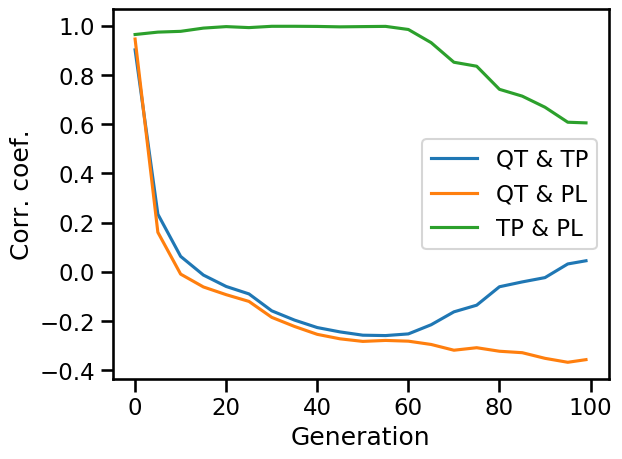
\includegraphics[width=\textwidth]{Figure/11-taxon_NSGAII_corr_plot}
			\caption{NSGAII: 11-taxon}
			%\label{fig:con_pr07}
		\end{subfigure}%
		\begin{subfigure}[b]{0.3\textwidth}
			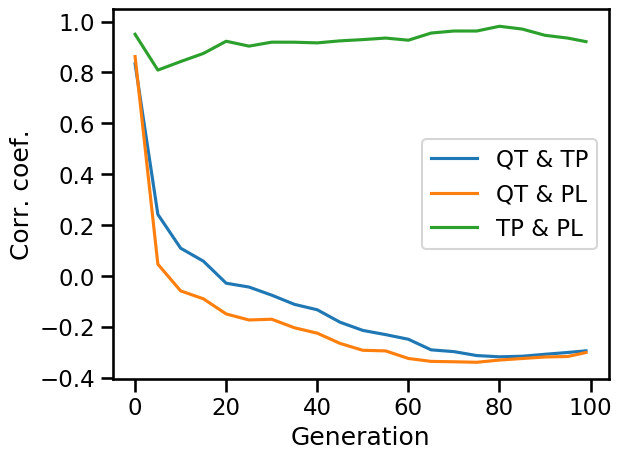
\includegraphics[width=\textwidth]{Figure/15-taxon_NSGAII_corr_plot}
			\caption{NSGAII: 15-taxon}
			%\label{fig:con_pr09}
		\end{subfigure}    
		\begin{subfigure}[b]{0.3\textwidth}
			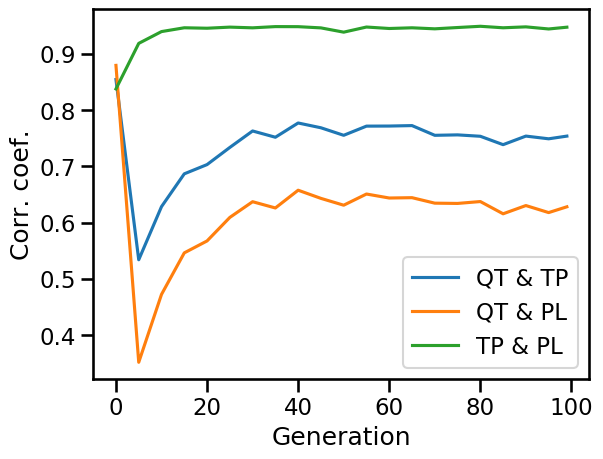
\includegraphics[width=\textwidth]{Figure/10-taxon_NOSSGA_corr_plot}
			\caption{SNOGA: 10-taxon}
			%\label{fig:con_pr06}
		\end{subfigure}%
		\begin{subfigure}[b]{0.3\textwidth}
			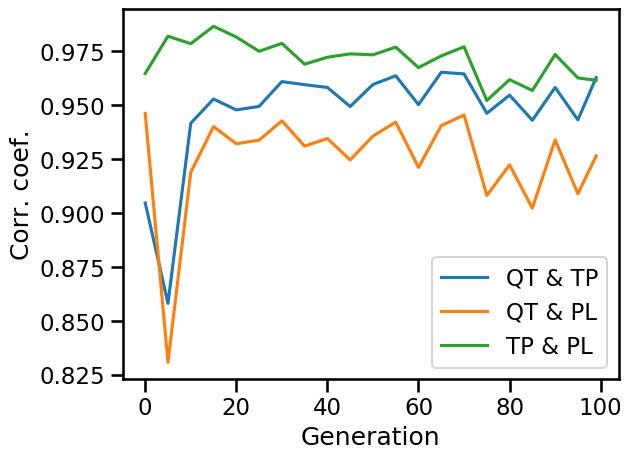
\includegraphics[width=\textwidth]{Figure/11-taxon_NOSSGA_corr_plot}
			\caption{SNOGA: 11-taxon}
			%\label{fig:con_pr07}
		\end{subfigure}%
		\begin{subfigure}[b]{0.3\textwidth}
			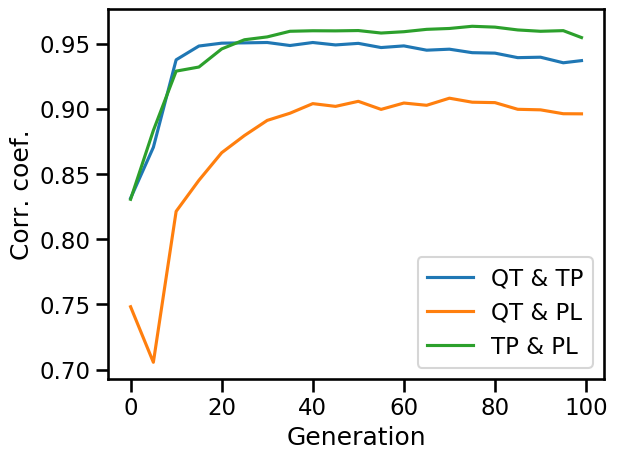
\includegraphics[width=\textwidth]{Figure/15-taxon_NOSSGA_corr_plot}
			\caption{SNOGA: 15-taxon}
			%\label{fig:con_pr09}
		\end{subfigure}
		\caption{Correlations between each pair of objectives against generations for NSGAII and SNOGA on three datasets.}
		\label{fig:gen_wise_correlation}
	%\end{adjustwidth}
\end{figure*}

\subsubsection{Correlation between two objectives} We plot the correlation coefficients between each pair of objectives against different generations for NSGAII and SNOGA on three datasets in Fig.~\ref{fig:gen_wise_correlation}. Here the horizontal axis represents the generations and the vertical axis represents the correlation coefficients averaged over 15 runs and 10 replicates. We see that, contrary to NSGAII, SNOGA does not exhibit any negative correlation coefficient between any pair of objectives. These results suggest that SNOGA is able to prevent the optimization of one objective to a great extent even at the loss of some other objectives, thereby alleviating issue~\ref{item:i1} (mentioned in Section~\ref{sec:problem}) to some extent.% as an attempt to resolve  (please see Section~\ref{sec:problem}) as we discussed earlier in Section~\ref{sec:method}). %objective to a great extent according to our requirement\footnote{Nayeem link it to the method section in algo}. 

\begin{figure*}[!htbp]
	\centering
	%\begin{adjustwidth}{}{}
		\begin{subfigure}[b]{0.3\textwidth}
			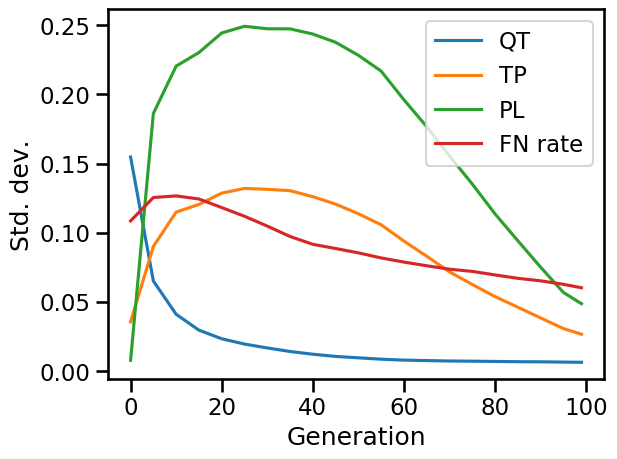
\includegraphics[width=\textwidth]{Figure/10-taxon_NSGAII_std_dev}
			\caption{NSGAII: 10-taxon}
			%\label{fig:con_pr06}
		\end{subfigure}%
		\begin{subfigure}[b]{0.3\textwidth}
			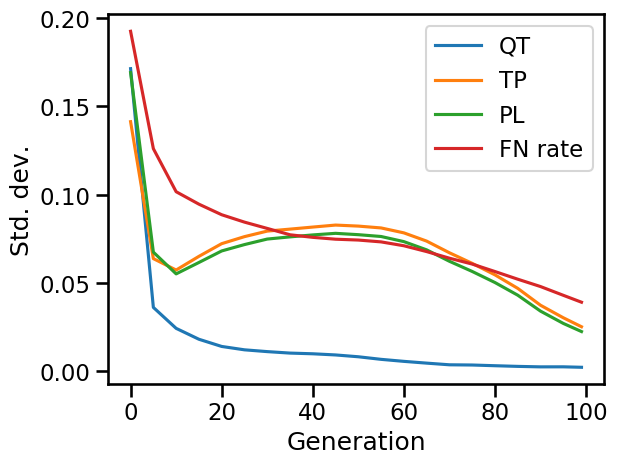
\includegraphics[width=\textwidth]{Figure/11-taxon_NSGAII_std_dev}
			\caption{NSGAII: 11-taxon}
			%\label{fig:con_pr07}
		\end{subfigure}%
		\begin{subfigure}[b]{0.3\textwidth}
			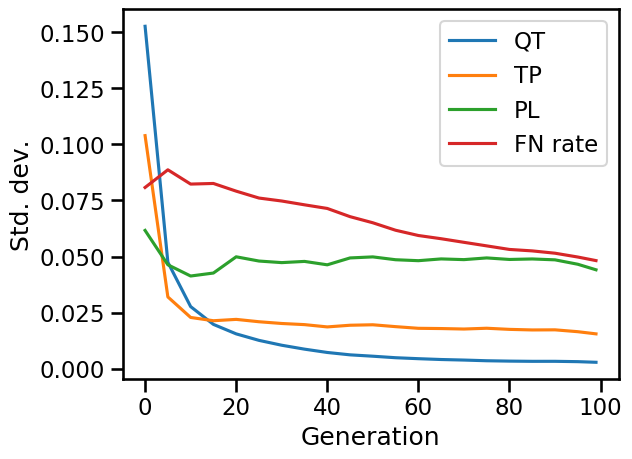
\includegraphics[width=\textwidth]{Figure/15-taxon_NSGAII_std_dev}
			\caption{NSGAII: 15-taxon}
			%\label{fig:con_pr09}
		\end{subfigure}
		\begin{subfigure}[b]{0.3\textwidth}
			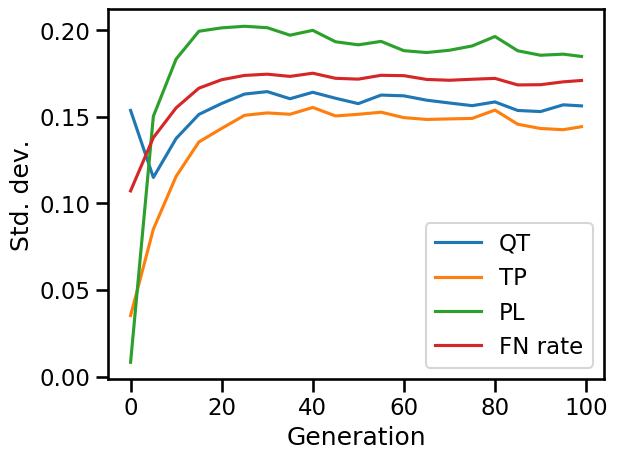
\includegraphics[width=\textwidth]{Figure/10-taxon_NOSSGA_std_dev}
			\caption{SNOGA: 10-taxon}
			%\label{fig:con_pr06}
		\end{subfigure}%
		\begin{subfigure}[b]{0.3\textwidth}
			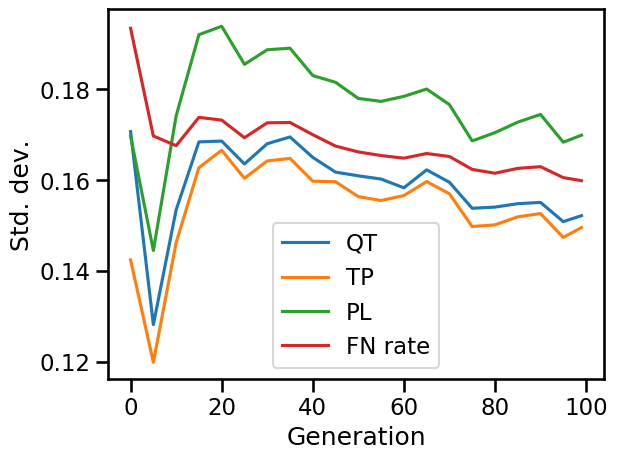
\includegraphics[width=\textwidth]{Figure/11-taxon_NOSSGA_std_dev}
			\caption{SNOGA: 11-taxon}
			%\label{fig:con_pr07}
		\end{subfigure}%
		\begin{subfigure}[b]{0.3\textwidth}
			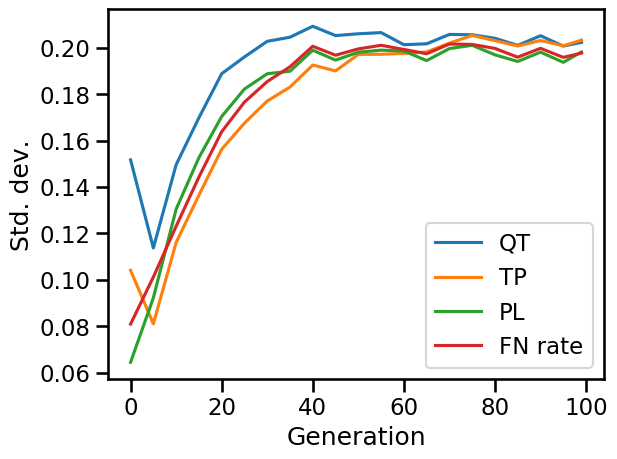
\includegraphics[width=\textwidth]{Figure/15-taxon_NOSSGA_std_dev}
			\caption{SNOGA: 15-taxon}
			%\label{fig:con_pr09}
		\end{subfigure}
		\caption{Variation of standard deviation of three objectives and FN rates in the population with generations for NSGAII and SNOGA on three datasets.}
		\label{fig:gen_wise_std_dev}
	%\end{adjustwidth}
\end{figure*}

\subsubsection{Diversity of objectives and FN rate}\label{subsubsec:diversity} Fig.~\ref{fig:gen_wise_std_dev} shows the variation of the standard deviation of three objective values (normalized using global maximum and minimum) of the population members and their respective FN rates in the population with generations for NSGAII and SNOGA on three datasets. Along the vertical axis, we plotted the standard deviation values averaged over 15 runs and 10 replicates. We find that SNOGA can maintain diversity throughout the generations presumably owing to the steps taken to mitigate issue~\ref{item:i2} which we discussed in Section~\ref{sec:method}. On the other hand, NSGAII loses diversity at an early stage.
%These figures clearly show that NSGAII loses diversity at an early stage possibly. This an outcome of not taking necessary measures to tackle issue~\ref{item:i2}~\cite{qu2010multi}. \footnote{The knowledge of FN rate is absent to the EMOs.}   

\begin{figure*}[!h]
	\centering
	%\begin{adjustwidth}{-1cm}{-1cm}
		\begin{subfigure}[b]{0.3\textwidth}
			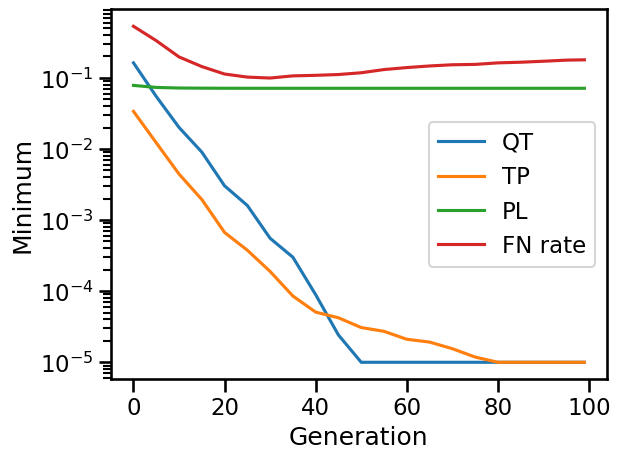
\includegraphics[width=\textwidth]{Figure/10-taxon_NSGAII_minimum}
			\caption{NSGAII: 10-taxon}
			%\label{fig:con_pr06}
		\end{subfigure}%
		\begin{subfigure}[b]{0.3\textwidth}
			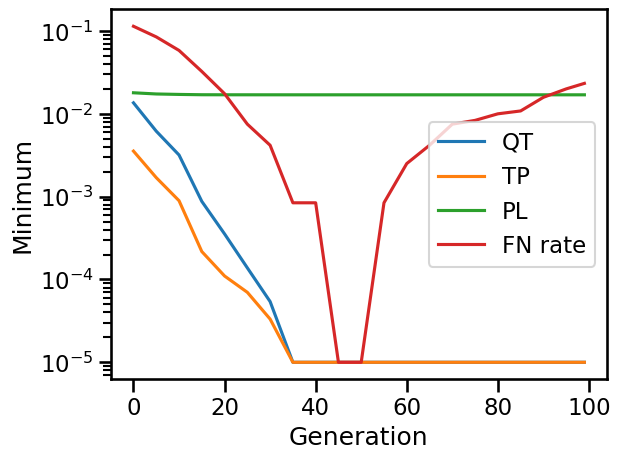
\includegraphics[width=\textwidth]{Figure/11-taxon_NSGAII_minimum}
			\caption{NSGAII: 11-taxon}
			%\label{fig:con_pr07}
		\end{subfigure}%
		\begin{subfigure}[b]{0.3\textwidth}
			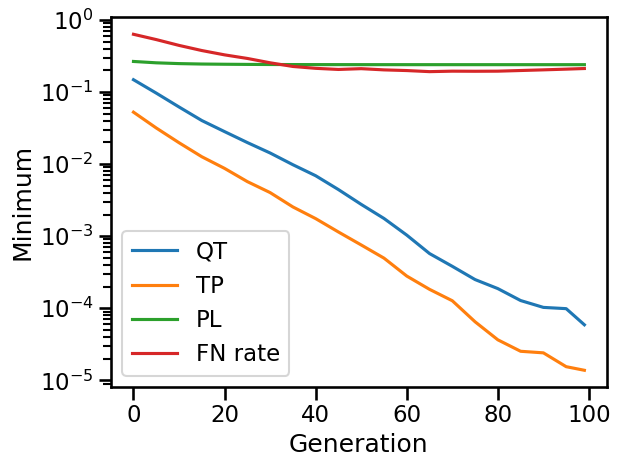
\includegraphics[width=\textwidth]{Figure/15-taxon_NSGAII_minimum}
			\caption{NSGAII: 15-taxon}
			%\label{fig:con_pr09}
		\end{subfigure}
		\begin{subfigure}[b]{0.3\textwidth}
			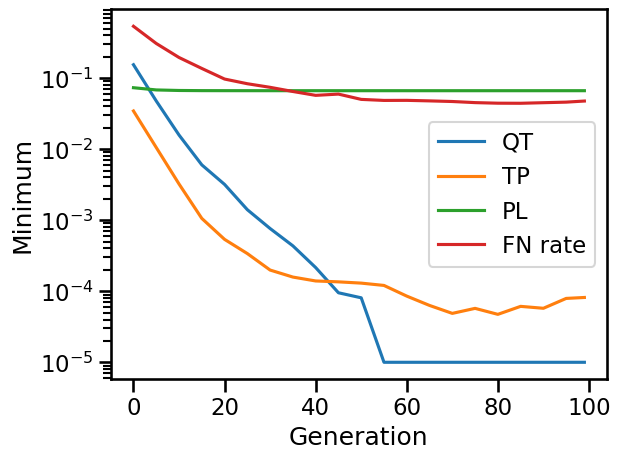
\includegraphics[width=\textwidth]{Figure/10-taxon_NOSSGA_minimum}
			\caption{SNOGA: 10-taxon}
			%\label{fig:con_pr06}
		\end{subfigure}%
		\begin{subfigure}[b]{0.3\textwidth}
			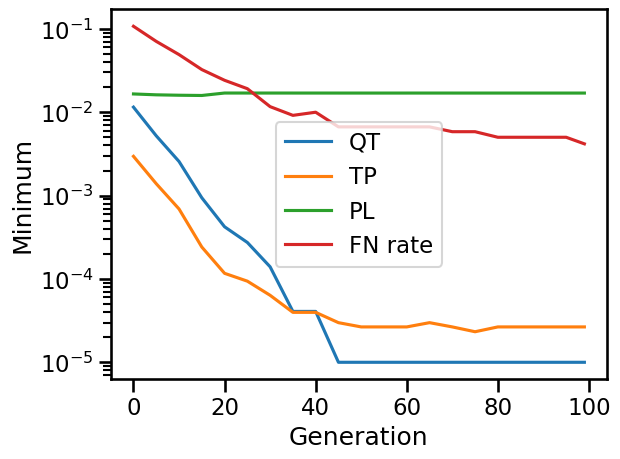
\includegraphics[width=\textwidth]{Figure/11-taxon_NOSSGA_minimum}
			\caption{SNOGA: 11-taxon}
			%\label{fig:con_pr07}
		\end{subfigure}%
		\begin{subfigure}[b]{0.3\textwidth}
			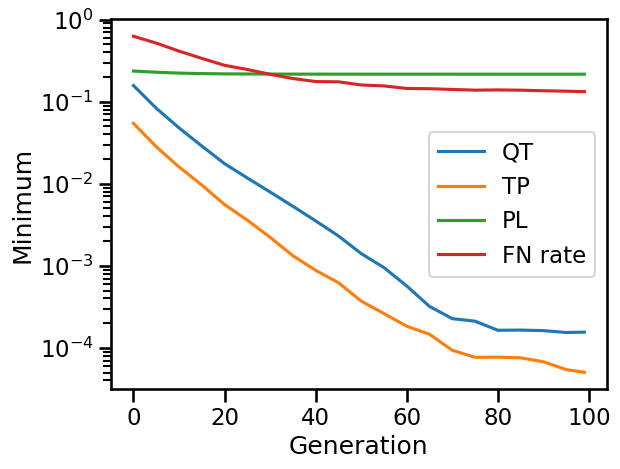
\includegraphics[width=\textwidth]{Figure/15-taxon_NOSSGA_minimum}
			\caption{SNOGA: 15-taxon}
			%\label{fig:con_pr09}
		\end{subfigure}
		\caption{Variation of minimum of three objectives (individually) and FN rates in the population with generations for NSGAII and SNOGA on three datasets.	}
		\label{fig:gen_wise_min}
	%\end{adjustwidth}
\end{figure*}

\subsubsection{Improvement of FN rate vs. individual objectives} Now we observe how the best (minimum) value of three objectives (individually) and FN rate (lower is better) in the population behave across generations for NSGAII and SNOGA as depicted in Fig.~\ref{fig:gen_wise_min}. The plotted values are averaged over 15 runs and 10 replicates. We mentioned earlier that FN rate reflects the true performance of an algorithm. However, the FN rate is not the fitness criterion of the optimization process. Rather, the optimization continues based on the three objective values (QT, TP and PL).
%But its knowledge is absent to the algorithm.
We see that, NSGAII allows one or more objectives to improve as much as possible which may cause the resultant species tree to deviate from the true tree (issue~\ref{item:i1}). As a result, the best FN rate of NSGAII starts to degrade after a particular generation despite continuous improvement of some objectives. For example, in Fig.~\ref{fig:gen_wise_min}(a), NSGAII achieves the best FN rate at around $ 30^{th} $ generation. Afterwards, the FN rate starts to degrade. However, QT and TP continue to improve until $ 50^{th} $ and $ 80^{th} $ generation respectively.
On the other hand, to avoid such deviation, SNOGA in effect, restricts the improvement of one or more objectives after certain number of generation. So its FN rate continues to improve. From these results, we can see that SNOGA is more effective than NSGAII in dealing with issue~\ref{item:i1}.%(except PL\footnote{To decrease the large runtime of PL calculation using MP-EST, we decreased the default iteration count})


\subsubsection{Comparison based on hypervolume} We mentioned in Section~\ref{sec:problem} that the problem that we deal with in this paper is different from the traditional MOPs. Importantly, the definition of convergence for MOPs is not the same as the convergence within the context of this problem. To explore this issue, we compare NSGAII and SNOGA in terms of hypervolume (HV)~\cite{zitzler1999multiobjective} which is probably the most popular performance measure used for MOPs. HV captures both convergence and diversity of the PF, sampled by an EMO algorithm, in a single real-value. For MOPs with all minimization objectives, a higher value of HV is desirable. In Fig.~\ref{fig:gen_wise_hv}, we plot the HV values for NSGAII and SNOGA which are averaged over 15 runs and 10 replicates. From these results, it is difficult to differentiate between these two algorithms. Both HV values get saturated at an early generation. Even, according to HV, SNOGA seems better than NSGAII more strikingly so for the larger dataset. The reason for worse value of NSGAII concerning HV could be attributed to the loss of diversity, as exhibited by it, at an early stage. 

\begin{figure*}[!htbp]
	\centering
	%\begin{adjustwidth}{-1cm}{-1cm}
		\begin{subfigure}[b]{0.3\textwidth}
			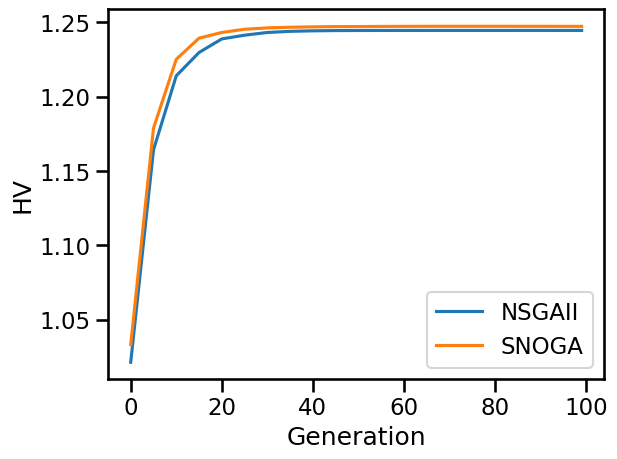
\includegraphics[width=\textwidth]{Figure/10-taxon_hv}
			\caption{10-taxon}
			%\label{fig:con_pr06}
		\end{subfigure}%
		\begin{subfigure}[b]{0.3\textwidth}
			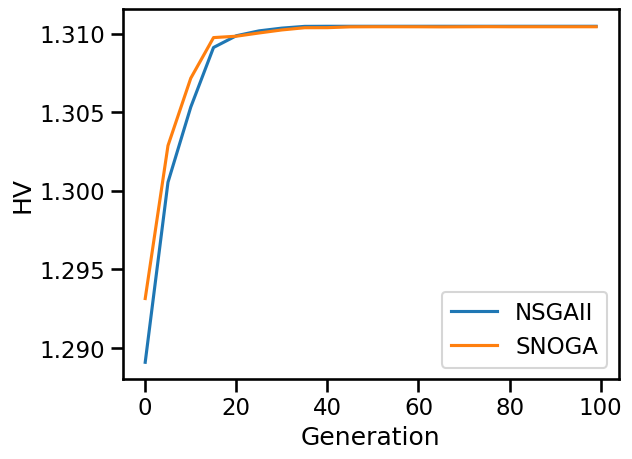
\includegraphics[width=\textwidth]{Figure/11-taxon_hv}
			\caption{11-taxon}
			%\label{fig:con_pr07}
		\end{subfigure}%
		\begin{subfigure}[b]{0.3\textwidth}
			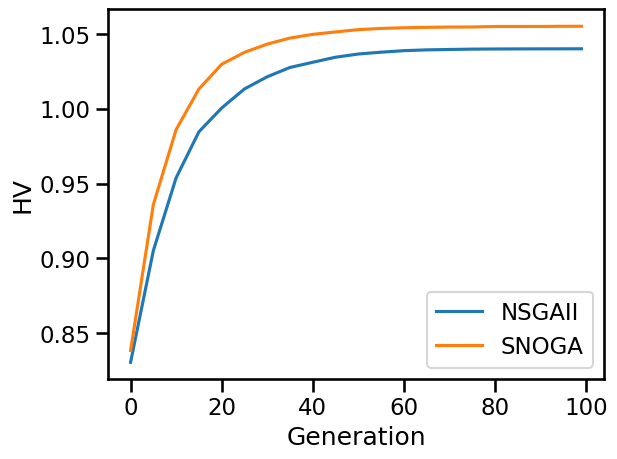
\includegraphics[width=\textwidth]{Figure/15-taxon_hv}
			\caption{15-taxon}
			%\label{fig:con_pr09}
		\end{subfigure}
		\caption{Variation of HV with generations for NSGAII and SNOGA on three datasets.}
		\label{fig:gen_wise_hv}
	%\end{adjustwidth}
\end{figure*}

\begin{figure*} [!htbp]
	\centering
	\begin{adjustwidth}{-0cm}{-0cm}
		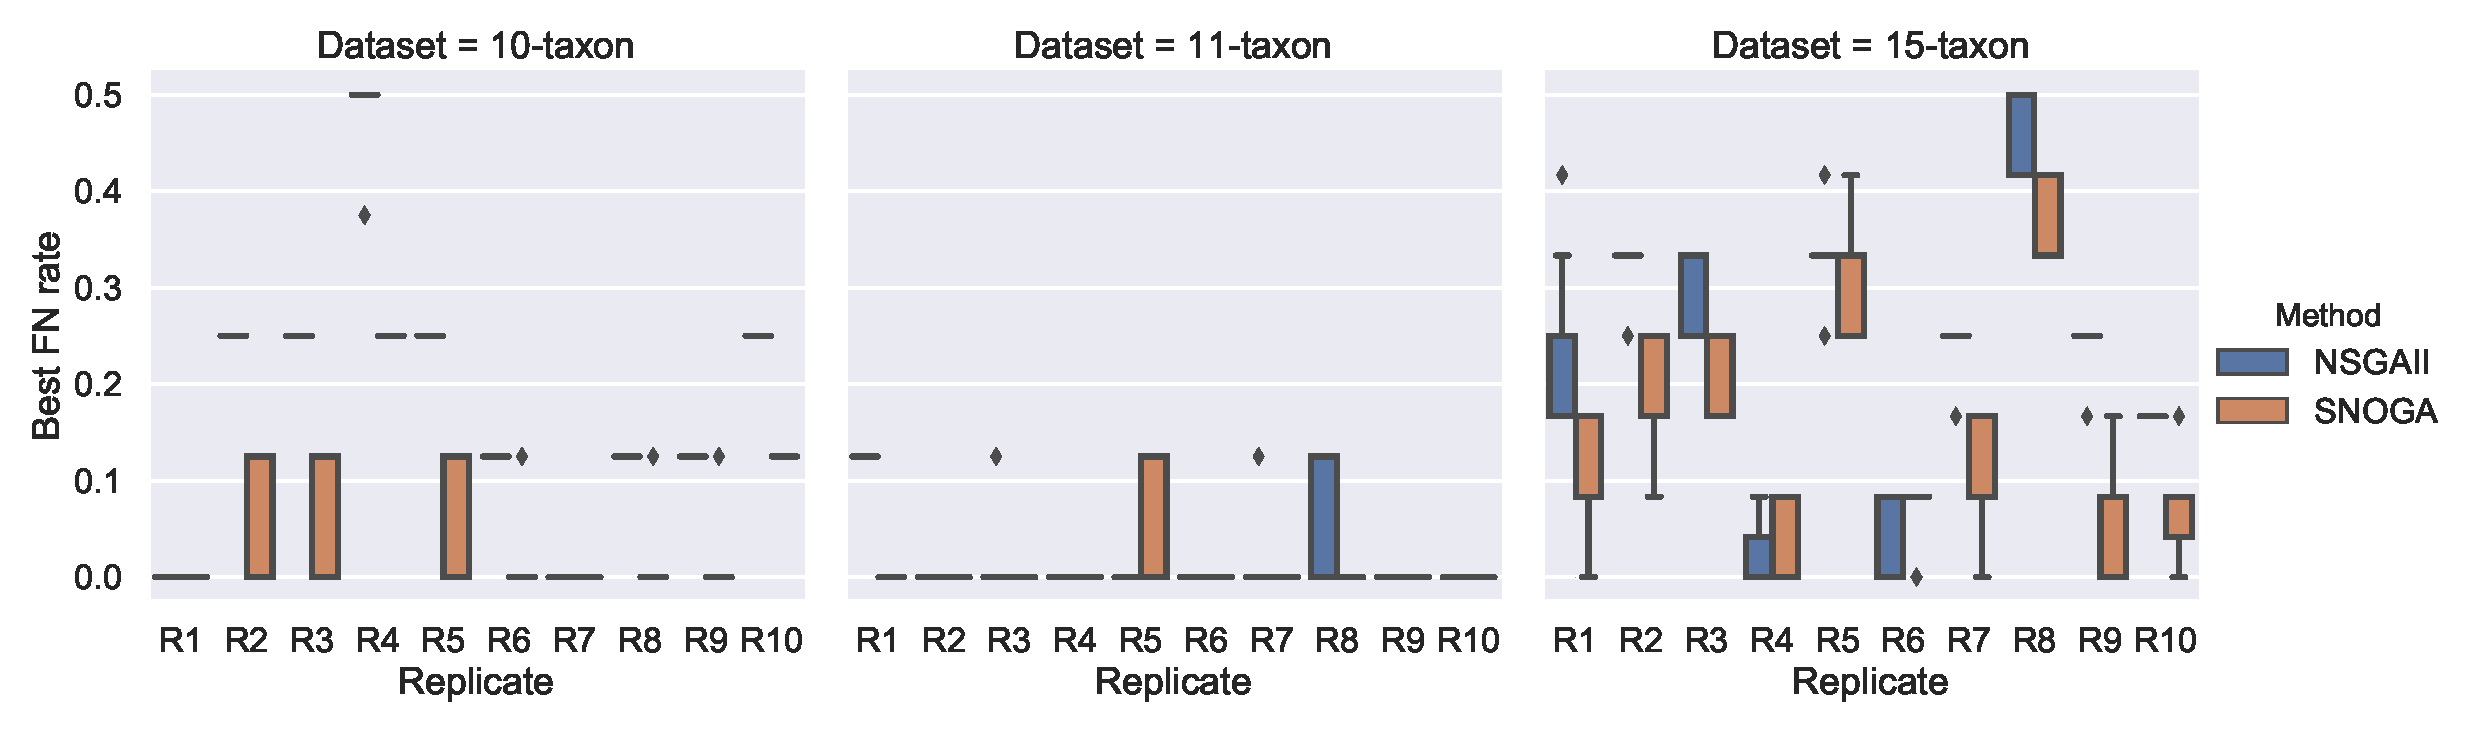
\includegraphics[width=1\textwidth]{Figure/emo_boxplot}
	\end{adjustwidth}
	\caption{Accuracy of the best estimated species trees extracted from the final population of NSGAII and SNOGA on each dataset having 10 replicate.} \label{fig:emo_compare}	
\end{figure*}


\npdecimalsign{.}
\nprounddigits{4}
% Table generated by Excel2LaTeX from sheet 'Sheet1'
\begin{table}[htbp]
	\centering
	\caption{Summary of FN rates achieved by NSGAII and SNOGA on 10 replicates of three datasets over 15 independent runs.}
	\begin{tabular}{|c|l|n{1}{1}|n{1}{1}||n{1}{1}|n{1}{1}|}
		\hline
		\multirow{2}{*}{Dataset} & \multicolumn{1}{c|}{\multirow{2}{*}{Rep.}} & \multicolumn{2}{c||}{NSGAII} & \multicolumn{2}{c|}{SNOGA} \\
		\cline{3-6}          &       & \multicolumn{1}{l|}{Average} & \multicolumn{1}{l||}{Std. Dev.} & \multicolumn{1}{l|}{Average} & \multicolumn{1}{l|}{Std. Dev.} \\
		\hline
		\multirow{10}{*}{10-taxon} & R1    & 0     & 0     & 0     & 0 \\
		\cline{2-6}          & R2    & 0.25  & 0     & 0.0583333 & 0.062360956 \\
		\cline{2-6}          & R3    & 0.25  & 0     & 0.0666667 & 0.062360956 \\
		\cline{2-6}          & R4    & 0.4916667 & 0.031180478 & 0.25  & 0 \\
		\cline{2-6}          & R5    & 0.25  & 0     & 0.05  & 0.061237244 \\
		\cline{2-6}          & R6    & 0.125 & 0     & 0.0083333 & 0.031180478 \\
		\cline{2-6}          & R7    & 0     & 0     & 0     & 0 \\
		\cline{2-6}          & R8    & 0.125 & 0     & 0.0166667 & 0.042491829 \\
		\cline{2-6}          & R9    & 0.125 & 0     & 0.0083333 & 0.031180478 \\
		\cline{2-6}          & R10   & 0.25  & 0     & 0.125 & 0 \\
		\hline \hline
		\multirow{10}{*}{11-taxon} & R1    & 0.125 & 0     & 0     & 0 \\
		\cline{2-6}          & R2    & 0     & 0     & 0     & 0 \\
		\cline{2-6}          & R3    & 0.0166667 & 0.042491829 & 0     & 0 \\
		\cline{2-6}          & R4    & 0     & 0     & 0     & 0 \\
		\cline{2-6}          & R5    & 0     & 0     & 0.0416667 & 0.058925565 \\
		\cline{2-6}          & R6    & 0     & 0     & 0     & 0 \\
		\cline{2-6}          & R7    & 0.025 & 0.05  & 0     & 0 \\
		\cline{2-6}          & R8    & 0.0666667 & 0.062360956 & 0     & 0 \\
		\cline{2-6}          & R9    & 0     & 0     & 0     & 0 \\
		\cline{2-6}          & R10   & 0     & 0     & 0     & 0 \\
		\hline \hline
		\multirow{10}{*}{15-taxon} & R1    & 0.2166667 & 0.073282811 & 0.1111111 & 0.0496904 \\
		\cline{2-6}          & R2    & 0.3166667 & 0.033333333 & 0.1944444 & 0.049690399 \\
		\cline{2-6}          & R3    & 0.3055556 & 0.03928371 & 0.2166667 & 0.040824829 \\
		\cline{2-6}          & R4    & 0.0222222 & 0.036851387 & 0.0555556 & 0.03928371 \\
		\cline{2-6}          & R5    & 0.3333333 & 0.030429031 & 0.3111111 & 0.056655772 \\
		\cline{2-6}          & R6    & 0.0444444 & 0.041573971 & 0.0666667 & 0.033333333 \\
		\cline{2-6}          & R7    & 0.2444444 & 0.020786985 & 0.1333333 & 0.050917508 \\
		\cline{2-6}          & R8    & 0.4611111 & 0.041573971 & 0.3777778 & 0.041573971 \\
		\cline{2-6}          & R9    & 0.2444444 & 0.020786985 & 0.0555556 & 0.0496904 \\
		\cline{2-6}          & R10   & 0.1666667 & 0     & 0.0666667 & 0.045133547 \\
		\hline
	\end{tabular}%
	\label{tab:emo}%
\end{table}%

\subsubsection{Comparison based on Tree accuracy} Finally, we compare NSGAII and SNOGA in terms of the tree accuracy for 10 replicates of each dataset. We measure tree accuracy in terms of the FN rate. A lower value of the FN rate corresponds to higher accuracy. We visualize the FN rates of the best trees obtained from the final population of 15 independent runs using boxplots in Fig.~\ref{fig:emo_compare}. Also, we summarize these results in Table~\ref{tab:emo}. We observe that SNOGA can offer much better trees than NSGAII in most of the 30 instances, whereas NSGAII outperforms SNOGA only on three cases (11-taxon: R5; 15-taxon: R4, R6). In some situations, two algorithms perform equally. We performed a standard paired $ t $-test based on the average FN rates achieved by NSGAII and SNOGA  (reported in Table~\ref{tab:emo}; this data satisfies the condition of normality and homoscedasticity~\cite{sheskin2003handbook}) and found significant difference ($t$-statistic: 5.20080, $p$-value: 0.00001) between them.


\begin{figure} [htbp]
	%\begin{adjustwidth}{0cm}{0cm}
		\centering
		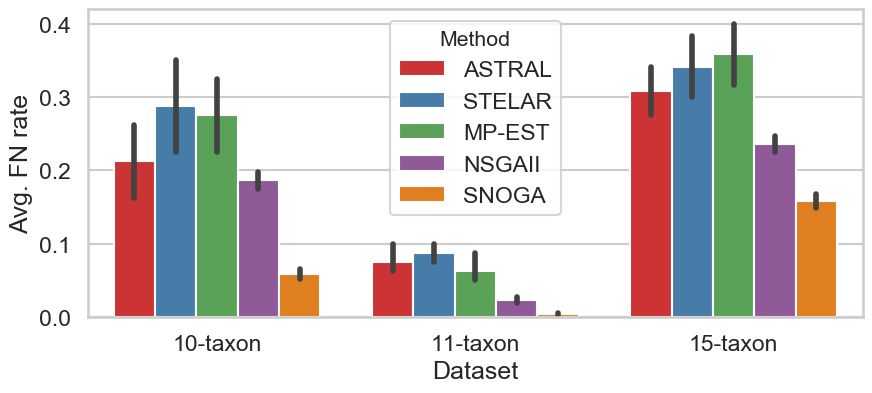
\includegraphics[width=0.5\textwidth]{Figure/all_dataset_compare}
		\caption{Performance comparison of ASTRAL, STELAR, MP-EST, NSGAII and SNOGA on three datasets. 
			%We show the average FN rates with standard error bars over 10 replicates
		} \label{fig:compare_exisitng_methods}
	%\end{adjustwidth}
\end{figure}

\subsection{Comparison with Existing Methods}
We evaluated the best trees offered by NSGAII and SNOGA in comparison with the output of ASTRAL, MP-EST and STELAR. On each dataset, we ran both NSGAII and SNOGA only for 99 generations (population size: 100, function evaluations: 10000). 
Fig.~\ref{fig:compare_exisitng_methods} shows the average FN rates with standard error bars over 10 replicates. We find that SNOGA offers the highest accuracy among all. On the 10-taxon dataset, SNOGA can achieve nearly 4X accuracy than ASTRAL. For the rest two datasets, the accuracy improvement is around 2X compared to ASTRAL. Interestingly, even the basic NSGAII exhibits more accuracy than the three existing methods. So the advantage of formulating this problem as a MOP is obvious. From actual application point of view, if we run the original NSGAII algorithm for a large number of generations its accuracy may fall for not resolving the issues mentioned in Section~\ref{sec:problem} properly which we saw earlier. Note that the FN rate is not the fitness criterion of the optimization process. Rather, the optimization continues based on the objective values.
So we can state that, owing to the characteristics designed considering the problem nature, SNOGA achieves at least 1.4X accuracy gain over the original NSGAII in all datasets. 



%\subsection{Discussion}

\begin{comment}
\begin{figure}[!htbp]
\centering
\begin{adjustwidth}{-1cm}{}
\begin{subfigure}[b]{0.55\textwidth}
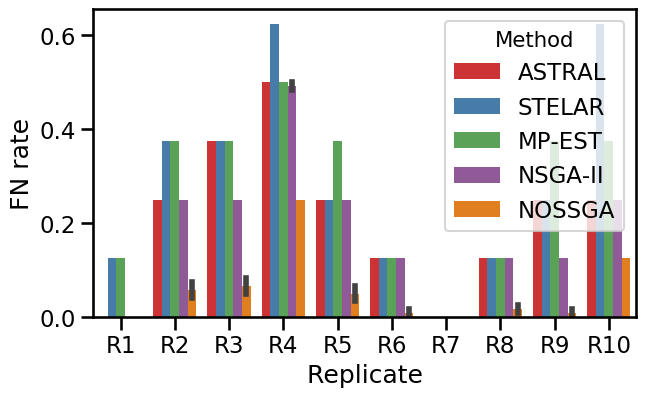
\includegraphics[width=\textwidth]{Figure/10-taxon_10_replicates}
\caption{10-taxon}
%\label{fig:con_pr06}
\end{subfigure}%
\begin{subfigure}[b]{0.55\textwidth}
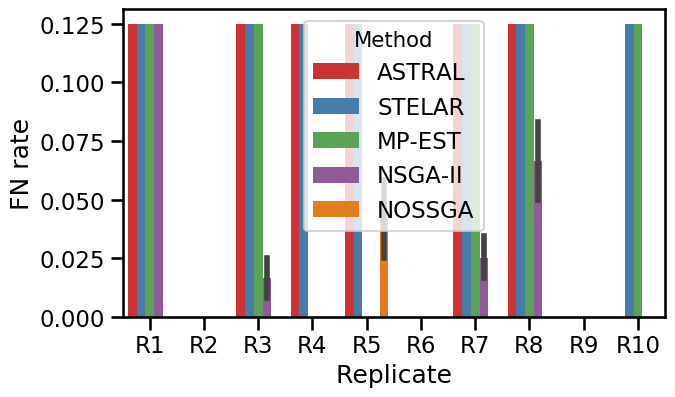
\includegraphics[width=\textwidth]{Figure/11-taxon_10_replicates}
\caption{11-taxon}
%\label{fig:con_pr07}
\end{subfigure}%
%    \newline

\begin{subfigure}[b]{0.55\textwidth}
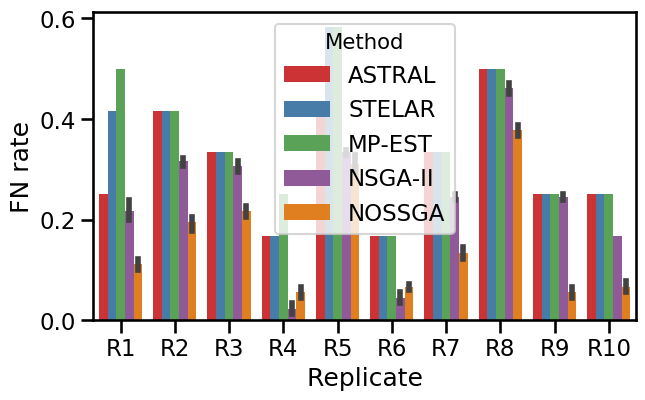
\includegraphics[width=\textwidth]{Figure/15-taxon_10_replicates}
\caption{15-taxon}
%\label{fig:con_pr09}
\end{subfigure}
\begin{subfigure}[b]{0.55\textwidth}
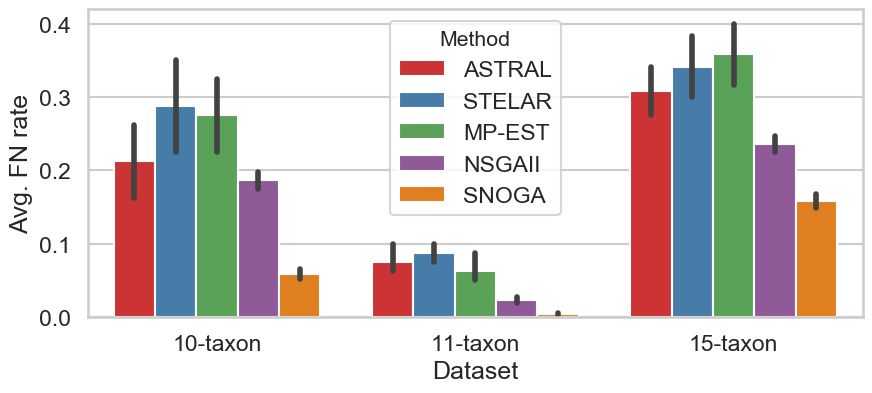
\includegraphics[width=\textwidth]{Figure/all_dataset_compare}
\caption{Summary}
%\label{fig:con_pr09}
\end{subfigure}%

\caption{Comparison of ASTRAL, STELAR, MP-EST, NSGAII and SNOGA on 10 replicates of 3 datasets.}
\label{fig:datasets}
\end{adjustwidth}
\end{figure}



\begin{figure}[!htbp]
\centering
\begin{adjustwidth}{-1cm}{}
\begin{subfigure}[b]{0.48\textwidth}
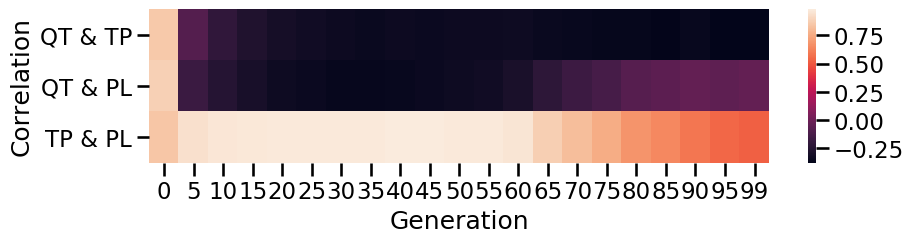
\includegraphics[width=\textwidth]{Figure/10-taxon_NSGA-II_heatmap}
\caption{NSGAII: 10-taxon}
%\label{fig:con_pr06}
\end{subfigure}%
\begin{subfigure}[b]{0.4\textwidth}
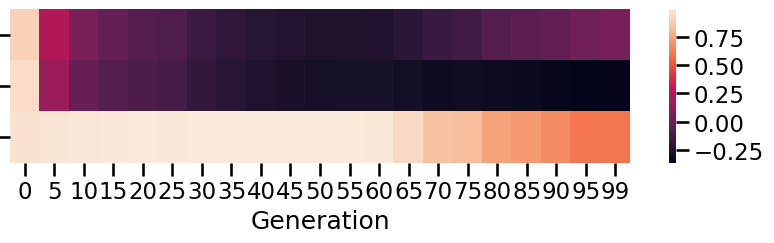
\includegraphics[width=\textwidth]{Figure/11-taxon_NSGA-II_heatmap}
\caption{NSGAII: 11-taxon}
%\label{fig:con_pr07}
\end{subfigure}%
\begin{subfigure}[b]{0.4\textwidth}
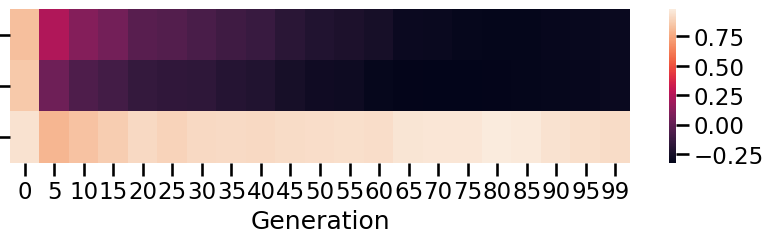
\includegraphics[width=\textwidth]{Figure/15-taxon_NSGA-II_heatmap}
\caption{NSGAII: 15-taxon}
%\label{fig:con_pr09}
\end{subfigure}

\begin{subfigure}[b]{0.48\textwidth}
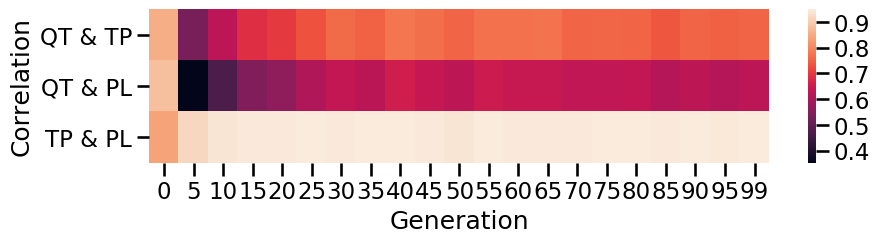
\includegraphics[width=\textwidth]{Figure/10-taxon_NOSSGA_heatmap}
\caption{SNOGA: 10-taxon}
%\label{fig:con_pr06}
\end{subfigure}%
\begin{subfigure}[b]{0.4\textwidth}
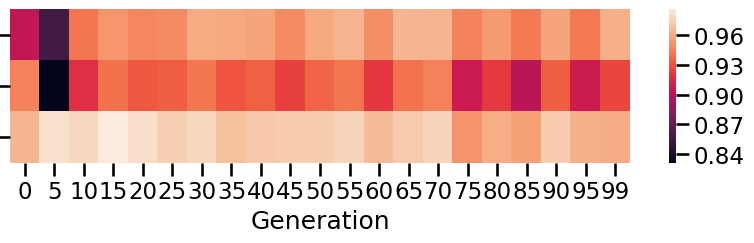
\includegraphics[width=\textwidth]{Figure/11-taxon_NOSSGA_heatmap}
\caption{SNOGA: 11-taxon}
%\label{fig:con_pr07}
\end{subfigure}%
\begin{subfigure}[b]{0.4\textwidth}
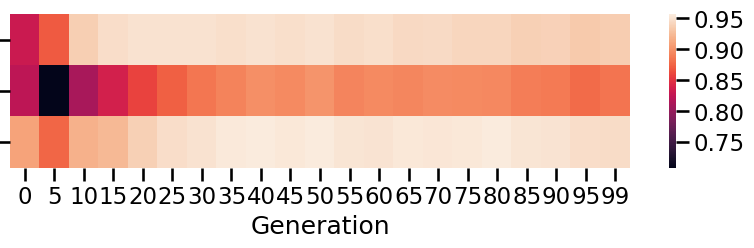
\includegraphics[width=\textwidth]{Figure/15-taxon_NOSSGA_heatmap}
\caption{SNOGA: 15-taxon}
%\label{fig:con_pr09}
\end{subfigure}
\caption{Correlation between each pair of objectives as the generation of an EMO progresses. For each dataset, we average the correlation coefficient over 15 runs and 10 replicates.}
\label{fig:gen_wise_correlation}
\end{adjustwidth}
\end{figure}
%\begin{figure}
%    \centering
%    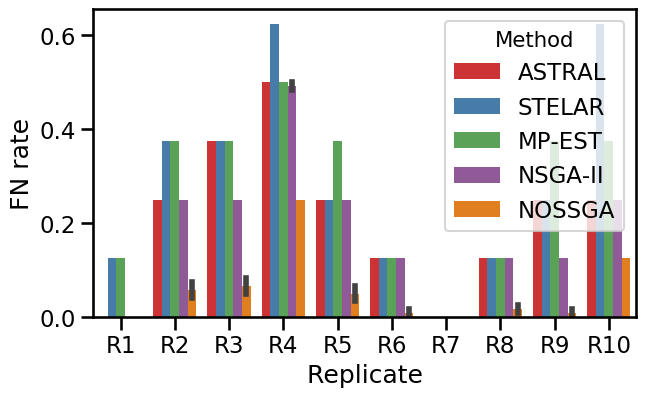
\includegraphics[width=0.6\textwidth]{Figure/10-taxon_10_replicates}
%    \caption{10-taxon.} \label{fig1}
%\end{figure}
%\begin{figure}
%    \centering
%    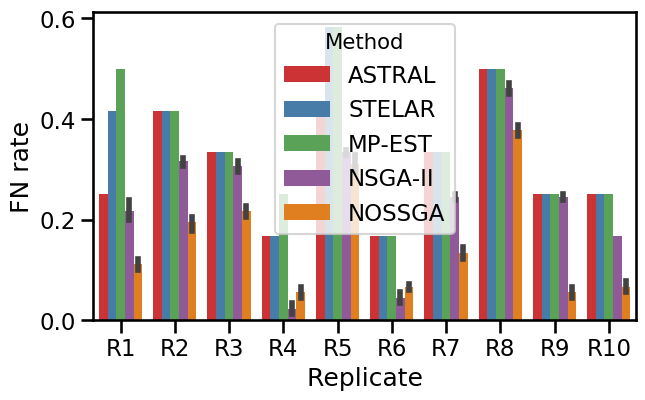
\includegraphics[width=0.6\textwidth]{Figure/15-taxon_10_replicates}
%    \caption{15-taxon.} \label{fig2}
%\end{figure}
\subsection{Results on 10-taxon dataset}
\subsection{Results on 11-taxon dataset}
\subsection{Results on 15-taxon dataset}
\end{comment}


\section{Conclusion} % and Future Work
In this paper, we have introduced the problem of estimating species trees from a set of gene trees as an MOP. We have shown examples where the existing method, optimizing a single criterion, can overshoot the criterion and thus deviate from the true species tree. We have selected three objectives from three existing methods. Unlike traditional MOPs, optimizing an objective beyond a certain limit and discarding a dominated at an early generation can reduce the chance of generating better trees. Hence we cannot expect PF, sampled by a classical EMO algorithm, to contain highly accurate trees. Therefore, we have designed a specialized EMO algorithm, namely, SNOGA, which is a modification of NSGAII. %We have shown that SNOGA can generate a tree-space containing highly accurate trees. 
We have analyzed the behavioral difference between SNOGA and NSGAII on a collection of challenging simulated datasets and found that the best trees offered by SNOGA are much better than the best trees generated by NSGAII. Finally, we have shown that the tree-space generated by SNOGA contains highly accurate trees in comparison with widely used methods that optimize a single criterion. We are currently working to devise a systematic methodology to extract a limited number of relatively better trees from the final population without the knowledge of the true tree to effectively process biological datasets. Besides, we are modifying another popular EMO algorithm, namely, MOEA/D, to effectively solve this problem.

%We are currently working to improve SNOGA so that it can efficiently process large biological datasets. 

%Finally, we found the accuracy of the best trees offered by SNOGA is quite better three existing methods on a collection of challenging simulated datasets. 

%We are currently working to devise a systematic methodology to filter a limited number of better trees from the final population without the knowledge of the true tree provided with the simulated dataset. At present, our mutation selects one from NNI/SPR/TBR at random with equal probability. As a future improvement, we will improve it by adaptively adjusting the selection probabilities based on the success rate of an operator in the previous generation. Also, we are planning to emded domain knowledge inside NNI, SPR and TBR so that they can make informed (as opposed to random) rearrangement in the given tree. To enable SNOGA processing large datasets within a reasonable time, we will improve the efficiency of objective evaluations. Moreover, we are modifying another popular EMO algorithm, namely, MOEA/D, to effectively solve this problem.



%
% ---- Bibliography ----
%
% BibTeX users should specify bibliography style 'splncs04'.
% References will then be sorted and formatted in the correct style.
%
\bibliographystyle{IEEEtran}
\bibliography{IEEEabrv,main_bib}

%\begin{subappendices}
\renewcommand{\thesection}{\Alph{section}}%
% or try \arabic{section}

\section{Also you should know this}
Really.
\section{And I also came across this}
But I need to put this in an appendix so that my paper is not too long.
\end{subappendices}
\end{document}
